%%%%%%%%%%%%%%%%%%%%%%%%%%%%%%%%%%%%%%%%%%%%%%%%%%%%%%%%%%%%%%%%%%%%%%%%%%%%%%%%%%%%%%%%%%%%%%%%%%%%

\chapter{The life of a molecular outflow from launching to fading}
\chaptermark{an outflow from launching to fading}
\label{chapter: joint discussion}


%%%%%%%%%%%%%%%%%%%%%%%%%%%%%%%%%%%%%%%%%%%%%%%%%%%%%%%%%%%%%%%%%%%%%%%%%%%%%%%%%%%%%%%%%%%%%%%%%%%%

The previous chapters each focus on specific aspects of the \ngc253 starburst: global properties of the molecular outflow (Chapter~\ref{chapter: outflow}), small-scale properties of individual molecular streamers (Chapter~\ref{chapter: outflow catalog}), physical and chemical environment of the forming super star clusters that power the starburst and outflow (Chapter~\ref{chapter: SSCs}), and finally a comparison with the Galactic center as a potential sibling of \ngc253 (Chapter~\ref{chapter: dendro}).
These chapters already included detailed discussions in the context of the respective literature. Therefore, the following sections will discuss higher level implications and how the separate aspects integrate into the life of an outflow from launching to fading.


\section{ALMA offers unprecedented resolution to study gas dynamics}

The primary dataset used in this thesis is the ALMA band~7 observations at $\sim 350$\,GHz that we conducted in cycles~3-4. The $\sim 8$\,GHz bandwidth covers dust continuum emission and a wealth of spectral lines of molecular species.
The unprecedented spatial resolution of 2.5\,pc is accompanied by a more than sufficient spectral resolution of 2.5\,\kms.
The large collecting area of ALMA allows to reach the required sensitivity in a short amount of time (on-source times: 12\,m extended: 3\,h~59\,min, 12\,m compact: 2\,h~37\,min, ACA: 14\,h~57\,min).

First of all, the data shown in this thesis are a first view into a new regime of nearby galaxy research. Observations such as these start to become routine work with finished, on-going and planned similar observations for other galaxies (e.g. \ngc4945 or Circinus).
These observations open nearby galaxy research to the methods of Galactic astronomy.
Before ALMA, parsec scale resolution could only be achieved regularly in the Milky Way and occasionally in the local group. The sensitivity to detect a whole correlator band filled with spectral lines required hundreds to thousands of hours of observation time and was therefore only feasible for a few selected targets.

The difficulties in calibrating and imaging the band~7 high-resolution dataset are only briefly mentioned in Chapters~\ref{chapter: outflow} to \ref{chapter: dendro} but show that we are currently operating at the forefront of the technical capabilities.
The comparison to and integration with literature data of lower resolution and other frequencies provides crucial additional information that are not yet available at matched quality (resolution and sensitivity).

The work detailed in the previous chapters and even simple figures such as the one on the cover illustrate the challenges but also the progress sparked by ALMA.
In that sense, the successful calibration, imaging and analysis of this dataset is a first major achievement of this thesis. In the diagnostically rich submillimeter regime, it shows for the first time a parsec scale view into the center of a nearby galaxy outside the local group.


\section{The complexity of molecular outflows in \ngc253}

Chapters~\ref{chapter: outflow} and \ref{chapter: outflow catalog} reveal the complexity of the molecular outflow in \ngc253 on parsec scales where previous observations only showed diffuse emission.
Such a detailed analysis of the molecular outflow is possible only thanks to the high spatial resolution of the ALMA \co32 data.

The molecular outflow in \ngc253 shows many small scale features of which 14 of the most striking ones are analyzed in Chapter~\ref{chapter: outflow catalog}.
Their distinct morphology, long but narrow and seemingly collimated features, raises questions about the launching mechanisms and geometry. Are these streamers actually collimated and if so, how? Probably more likely, they instead form from a continuous structure breaking up into pieces, somewhat similar to a sheet of water in a fountain that fractures into small streams.
Such questions can only be answered by high-resolution simulations in which the underlying physical mechanisms can be explored. While many simulations correctly predict the large scale and global properties of outflows, they differ in the predicted small scale structure and launching mechanisms \citep[e.g.][]{2010ApJ...709...27W,2017MNRAS.466.1903G,2018ApJ...853..173K,2020MNRAS.493.2149K,2019MNRAS.490.3234N,2019arXiv191009566M}.
At this point, the typical quantities inferred for size, mass or energetics of molecular streamers (Table~\ref{outflow catalog: table: outflow catalog}) provide crucial input to discern simulations.
Using the 3D position-position-velocity information of the streamers, it is possible to trace them back to the starburst and estimate their potential launching sites with $\LESSSIM 20$\,pc projected accuracy. Reassuringly, the estimated historic launching sites typically lie within $\sim 20$\,pc of sites of current star formation in massive molecular clumps and (proto-)SSCs.

Chapter~\ref{chapter: outflow} shows that although the streamers are striking in images, a significant amount ($\sim 50$\%) of luminosity or mass and therefore also relevant quantities of energy and momentum, are located in a diffuse molecular outflow.
Such a statement is only possible by applying a systematic definition of outflow to the data which then separates into a rotating disk component, an outflow component and another component of kinematically anomalous gas from various sources. Again, only the high spatial resolution of the \co32 data enables this analysis.
By applying the kinematic separation to literature data at lower resolution but larger field-of-view (\co10 and \co21), a comprehensive insight into the molecular outflow becomes possible.

The molecular outflow in \ngc253 is massive ($\sim 0.5 \times 10^8$\,M$_\odot$) and the associated mass flow rate dominates the mass rates of the other gas phases. At $\dot{M} = 14-39$\,\Msunyr, most likely $\dot{M} \sim 20$\,\Msunyr, the molecular outflow has a significantly higher mass outflow rate than the observed ionized outflow ($\sim 1$\,\Msunyr) and a potential neutral outflow but is also a factor $\eta=\dot{M}_\mathrm{SFR}/\dot{M}_\mathrm{out} = 14-20$ higher than the star formation rate. 
Similar values for mass loading factors $\eta$ have been found for other sources in the literature before but it still is surprising that a relatively weak starburst of $SFR = 1.7-2.8$\,\Msunyr \citep{Ott:2005il,Leroy:2015ds,2015MNRAS.450L..80B} can drive such a massive outflow.

Owing to its high gas mass, the kinetic energy of the molecular outflow is substantial, although it is slow compared to the ionized outflow. The $2.5-3.1 \times 10^{54}$\,erg in bulk kinetic energy and a similar amount in internal kinetic energy (velocity dispersion, most of which is turbulence) can be easily supplied by the starburst at its current SFR. Coupling efficiencies of $\sim 0.1$\% to the total or $\sim 8$\% to the kinetic feedback energy are sufficient to explain the bulk kinetic outflow energy.
The molecular outflow momentum of $4.8-6.4 \times 10^8$\,\Msunkms yields coupling efficiencies $\sim 2.5-4$\% to the momentum supplied by stellar feedback (SNe and winds) in \ngc253.
These numbers are generally difficult to measure but provide crucial information on the efficiency of stellar feedback in the context of galaxy evolution and in simulations.

It must be noted that despite the improved outflow identification which achieves higher precision than literature work, the results still have considerable uncertainties associated.
The intrinsic geometry of the outflow in \ngc253 is not yet known down to the required level of detail. The well-motivated basic picture of an outflow cone of layered gas phases cannot provide information on the exact location of each outflow feature. 
Furthermore, the observed gas distribution can be explained by a constant starting mass outflow rate over the lifetime of the starburst, through continuous gas ejection without acceleration of the gas after ejection, or a mixture of both mechanisms.
The degeneracies between unknown geometry and outflow history typically cause of order 0.5\,dex error. For individual features, more precise estimates may be possible by utilizing further information (e.g. line-of-sight location by absorption measurements) but for the molecular outflow as a whole significant uncertainties will remain.

With the data at hand, it is only possible to probe the outflow out to $\sim 340$\,pc from the estimated launching sites in the disk. Further out, the molecular outflow becomes too faint to be detected. Future observations at higher sensitivity may detect more widespread molecular outflows. The geometry of \ngc253, however, complicates this search as the projected southern spiral arm crosses the south-western edge of the extrapolated outflow cone. Unfortunately, this spatial coincidence occurs at exactly the extrapolated velocity of the outflow and a separation is impossible when based only on observational ppV data.
Therefore, more about the distant outflow may be learned from the other outflow phases (ionized, neutral), chemical/physical information within the gas and a better understanding of the interactions between the phases (cf. Section~\ref{discussion: section: outflow launching}).


\section{The kinematic environment of molecular gas in and outside a starburst}

\begin{figure}
    \centering
    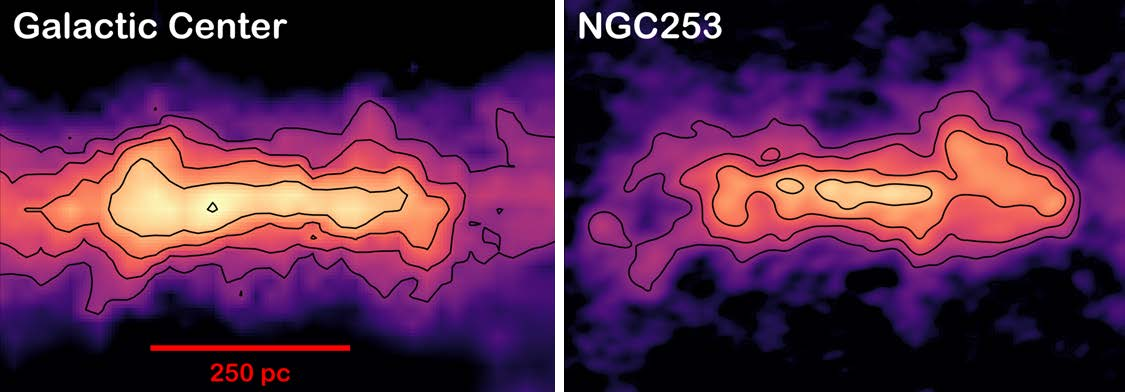
\includegraphics[width=\textwidth]{thesis/images/chapters/discussion/NGC253-GC_comparison.pdf}
    \caption[Comparison of the \co10 distribution in \ngc253 and the GC]{Comparison of the molecular gas traced by \co10 in \ngc253 \citep{2013Natur.499..450B} and the GC \citep{2001ApJ...547..792D}. The resolution has been matched to a common 32\,pc, set by the \ngc253 observations (Krieger et al. 2020b, submitted). The size scale of the images is identical in physical units. On GMC scales, the centers of \ngc253 and the GC look very much alike in the molecular gas distribution and structure. This similarity extends down to parsec scales as inferred from \co32 observations.
    }
    \label{discussion: figure: NGC253 GC comparison}
\end{figure}

The Milky Way's Galactic Center is surprisingly similar to the center of \ngc253 in many aspects. For instance, the (molecular) gas distribution (Figure~\ref{discussion: figure: NGC253 GC comparison}) is very similar and the overall structure is alike with a $\sim 200$\,pc ring and condensations along the ring in which massive star formation takes place. The striking difference, however, is the star formation activity: an ongoing starburst in \ngc253 \citep[$SFR = 1.7-2.8$\,\Msunyr][]{Ott:2005il,Leroy:2015ds,2015MNRAS.450L..80B} but relatively quiescent star formation \citep[$SFR \sim 0.1$\,\Msunyr;][]{2017MNRAS.469.2263B} in the GC. The availability of molecular gas alone cannot explain the factor ten difference in SFR as the total molecular gas masses differ by only a factor $\sim 2$.

Chapter~\ref{chapter: dendro} shows how these similarities and differences affect the kinematic state of the gas. 
The resolution-, area- and noise-matched data provide a direct comparison in two CO transitions, at two resolutions in the molecular gas.
The use of dendrograms as a standard structure identification technique allows for a consistent definition of kinematic parameters and a fair comparison between the environments.

Significant offsets in the size--line width relations show that the starburst in \ngc253 affects the (turbulent) linewidth of the gas. It is higher by a factor $\sim 2-3$ in \ngc253 than in the GC.
The more turbulent gas and therefore increased kinetic energy in the gas of \ngc253 is plausibly supplied by stellar feedback. 
The excess kinetic energy in \ngc253's molecular gas relative to the GC, together with the (bulk plus turbulent) kinetic energy in the molecular outflow requires only $20-25$\% of the kinetic feedback energy. Note, however, that this number is only a rough estimate and cannot be calculated exactly from the dendrogram data.

Aside from feedback, also variations in the gas structure could cause differences in the observed line widths.
In particular, the scaling of cloud mass or density with cloud radius could be different. More massive clouds need to be supported by higher turbulent pressure against collapse, otherwise they would collapse rapidly on a free-fall time and would hardly be observable during their short lifetime. 
Such effects would show in size--mass relations or mass (density) PDFs which is not observed. 
Hence, systematic differences of gas structure do not cause the broader line widths in \ngc253.

An examination of the virial state of the molecular gas reveals that especially low column density gas behaves differently in the two galaxies. The data implies a dominating external pressure $P_\mathrm{ext} = 10^7-10^{7.5}$\,K\,\pcm3 in \ngc253 that elevates linewidths in the low column density gas. In the GC, clouds are subject to a variety of external pressures and no collective effect shows in the virial state.
Gravitationally unbound, low column density gas present in \ngc253 but not in the GC strongly suggests that this gas is associated with the molecular outflow, in particular the diffuse molecular outflow, already discussed in Chapter~\ref{chapter: outflow}.
The virial state of the high column density gas marginally deviates between \ngc253 and the GC. This is surprising since star formation occurs in the highest (volume) density gas and therefore feedback impacts this gas first. Apparently, the dense, starforming gas is not as much affected by the starburst as the low density gas.

A wide comparison to the literature shows that \ngc253 and also GC behave relatively typical in the size, line width and mass (density) scaling relations compared to other Galactic and extra-galactic star forming environments.

Overall, differences in the kinematic state of the molecular gas cannot provide an easy explanation for the different SFR despite otherwise similar properties of the star forming gas in \ngc253 and the GC.
This lack of simple mechanisms to explain the different modes of star formation might be solved by models that go beyond stationary dynamical arguments of cloud stability and feedback regulated star formation.
Models of episodic star formation in galactic centers provide a potential solution \citep[e.g.][]{2015MNRAS.453..739K,2019MNRAS.484.1213S}.
The observed difference in star formation would then just be a sampling effect: We catch the GC in a quiescent phase with little star formation when it builds up mass for a later starburst. \ngc253 on the other hand, is currently observed during a burst phase and will go back to a quiescent phase once the reservoir of dense gas is exhausted.


\section{The complexity of molecular gas in (future) feedback sources}

To better understand the properties of the starburst and the gas in which it occurs, Chapter~\ref{chapter: dendro} zooms into the super star clusters in which most of the star formation in \ngc253 occurs \citep[up to 100\% of the starburst SFR;][]{2018ApJ...869..126L}.
Using once again the high-resolution band~7 data, Chapter~\ref{chapter: SSCs} presents highly complex spectra of the (proto-)SSCs. 
The single pixel ($0.1\arcsec \times 0.1\arcsec$ or 1.7\,pc $\times$ 1.7\,pc) spectra probe the $\sim 2-4$\,pc size scales of the SSCs due to smearing by the 2.5\,pc beam.
Up to 55 spectral lines of 14 species are detected in only 7.8\,GHz bandwidth (at $\sim 350$\,GHz) which creates complex blended composite spectra and requires line modelling with \xclass to disentangle. The modelling approach provides complementary observation-based quantities (line intensities, line ratios) and modelled physical quantities (column density, temperature).

The SSCs differ significantly in chemical complexity between 5 and 15 detected species, partially due to sensitivity limits of fainter sources and partially due to intrinsic chemical variations.
The classical (dense) molecular gas tracers CO, HCN, HCO$^+$ and CS show complex line profiles with multiple components and potential signs of (self-)absorption in four SSCs. Interestingly, all other species do not show relevant deviation from single Gaussian components.

The SSCs contain significant fractions of dense gas, implied by the line ratios CO/HCN and CO/HCO$^+ \sim 1-10$, as is expected for actively starforming environments.
The radiative energy source of the molecular gas in the SSCs are UV photons rather than X-rays which is shown by comparisons to different model predictions that favor PDRs over XDRs. 
The detection of bright HC$_3$N emission from highly excited states in many SSCs further implies high IR radiation fields and gas temperatures.
Therefore, PDRs cannot provide the overall dominant energy source. Instead, mechanical heating by in/outflows and turbulence is likely to be the dominant energy input into the gas, supported by weaker UV fields. 
Alternatively, the dense and therefore opaque gas shields different regions from each other in which different conditions co-exist spatially separated.

\ngc253 is thought to host a SMBH\footnote{There are no clear detections of a SMBH in \ngc253 yet because of extremely high extinction in the gas and no obvious detection of AGN activity. Kinematic arguments suggest $M \sim 7\times10^6 - 1.4\times10^7$\,\Msun \citep{2006ApJ...644..914R,2020MNRAS.tmp..289C} for a central compact mass and the $M-\sigma$ relation implies $M \sim 2\times10^7$\,\Msun \citep{2019A&A...623A..79C}.} that might influence the chemistry in close-by SSCs if it were to be actively accreting and providing feedback. The fact that none of the SSCs show signs of an XDR, places limits on the potential AGN luminosity or the geometry in the starburst is more complex than expected. \ngc253's SMBH remains elusive.

According to chemical models, several of the detected line ratios indicate dense gas at order $10^5$\pcm3 which is further supported by high optical depths even in typically optically thin isotopologs such as H$^{13}$CN and HC$^{15}$N.
The frequent detection of vibrationally excited lines of HCN and HC$_3$N indicate IR greenhouse conditions in the dense inner regions of the SSCs.
As can be expected for such an environment, the molecular gas in the SSCs is hot with $\sim130$\,K average SO$_2$ rotational temperature across the sources.

These results show a snapshot of the continuous interaction of massive, young (forming) clusters with the molecular gas in between and around the (forming) stars.
Some of the younger clusters will continue to accrete gas and gain stellar mass. Once the stellar feedback becomes strong enough, the remaining gas will be dispersed and a significant fraction may end up in future (molecular) outflows.



\section{The outflow life cycle}

Taken together, the Chapters~\ref{chapter: outflow} to \ref{chapter: dendro} trace the whole life cycle of a molecular outflow: from actively star forming gas prior to ejection by stellar feedback to parsec scale structures breaking out of the star forming disk to forming an outflow cone of hundreds of parsec in size.
From these studies, an observational view on the life of a molecular outflow in \ngc253 can be sketched out as follows.

Formed from dense, strongly irradiated gas that is left-over from cluster formation, molecular outflows are launched in or around those clusters.
Prior to and during launching of the gas, it is difficult to observe due to highly complex kinematics and absorption in and around the clusters. Blending with the surrounding molecular disk further complicates observations. Optically thin tracers are required but traditional extra-galactic tracers of common isotopologs (e.g. H$^{13}$CN and HC$^{15}$N) still suffer from significant optical depth. More rare isotopes, double isotopologs (e.g. $^{13}$C$^{18}$O) or less abundant complex molecules are better suited but place challenging constraints on sensitivity.

Shortly after being launched at timescales of $\LESSSIM 1$\,Myr, molecular outflows are easier to identify when they break out of the (projected) star forming disk. At sufficiently high resolution, their launching site can still be inferred kinematically with good ($\LESSSIM$ 20\,pc) accuracy.
In the meantime, when the outflowing gas is still blended with the disk, it shows as unbound gas with enhanced line widths in cloud decomposition analyses. Compared to the dense star forming clumps, it is at lower density.

On the smallest scales, the outflowing gas is likely driven spherically or over large solid angles (cf. mostly spherically symmetric \hii regions). The associated bubbles and superbubbles then merge and interact when growing. These tens of parsecs large structures are easily detectable even at low spatial resolution ($\GTR 30$\,pc) and in classical tracers such as CO \citep[e.g.][]{2006ApJ...636..685S,2013Natur.499..450B}.
The merging (super-)bubbles probably push the molecular gas to the sides resulting in a radially stratified outflow of an ionized core surrounded by molecular gas and potentially a neutral layer in between \citep[e.g.][]{Strickland:2002kp,2015ApJ...801...63M}.
This multi-phase outflow expands on its journey away from the disk which results in a cone-like structure. Given enough information on the geometry, the cone structure can be used to kinematically isolate outflowing gas.
The molecular layer on the outflow cone cannot be uniformly covered since feedback and outflow launching is a stochastic process. Furthermore, even a uniform outflow layer will at some point begin to fragment due to gravitational or radiative instabilities and interactions. At this stage, dozens to hundreds of parsec from the launching site, the molecular outflow might be better described as a collection of streamers on the surface of a cone. The SW streamer is the most impressive representative of this stage in \ngc253.
The space in between the locally overdense streamers may be filled by diffuse molecular gas. However, it is unclear how this could survive in a relatively thin sheet and in a highly irradiated environment (right next to the ionized outflow cone). Unresolved and blended (by projection or beam smearing) streamers may also give the impression of diffuse gas.
Limb brightening emphasizes the projected edges of the cone in observations and gives rise to a (partially filled) X-shaped signature.

In \ngc253, the molecular outflow can be traced out to $\sim300$\,pc in localized features (SW streamer) or $\sim 350$\,pc as a spectral feature (kinematic decomposition). 
Beyond that, the molecular gas might be destroyed (dissociation, ionization) or become too faint for detection, either by dispersion due to the growing surface of the expanding cone or because turbulent pressure within the streamer finally prevails over gravitational forces and external pressure.
The ionized and neutral outflow phases have been detected over much larger kpc scales, so it is plausible that the molecular outflow also extends further and is just not detected yet.

\vspace{\baselineskip}

The detailed high resolution picture that can be drawn for the \ngc253 outflow provides crucial background information for simulations aiming at understanding the physical processes behind outflows and the interpretation of lower resolution observations in the more distant universe.
Today, we can resolve the sites of star formation in a starburst, as this thesis has shown, but such an achievement is not possible for $z\sim1-2$ galaxies at the peak of the cosmic star formation history.
The observations presented here show a highly complex environment but comparisons with earlier lower resolution (tens to hundreds of pc) data show that the small scale gas properties are often not too far from the (extrapolated) large scale averages. Local effects on small spatial scales may, however, have significant impact in specific situations.
Therefore, the kpc resolution observations at $z\sim1-2$ need to consider the unresolved complexity but careful estimates of the small scale star formation process can be possible also from large scale averages.
